\documentclass[../main.tex]{subfiles}
\begin{document}
\subsection{Graphs are Matroids} 
\begin{thm}
\noindent Let $G$ be a graph and $\mathcal{I}$ be the set of all cyclefree subgraphs of G.
Show that if we have the pair $(E,\mathcal{I})$ as defined above by our graph, we have a matroid. In other words, that the cycle matroid $M(G)$ of a graph is a matroid.
\end{thm} 
\begin{proof}
 Let $A,B \in \mathcal{I}$ with $|A|=|B|+1.$
 \noindent To prove $ I3 $ of the definition of a \textit{matroid}, We show that for some $a \in A ,$\\$ B \cup \{a\} \in \mathcal{I},$  we should consider $B \cup \{a\}$ for each $a \in A.$ 
 
 \noindent Now suppose $ |A|  >  |B| $ and that $|A|  =  |B| + 1$\\
 Let 
 $ |A \cap B| = s $ , $ |A \setminus B| = r$ ,
 $ |A| = s + r $ and $ |B| = s + r - 1$ 
 
\noindent So $ |B \setminus A| = r - 1$
 
 \noindent Suppose $ A \setminus B = \{ a_1, a_2, .... , a_r \} $ 
 
 \noindent Suppose $ B \cup \{ a_i \} \notin \mathcal{I} \hspace{3mm} $ for each $ i \in \{ 1,2,... \}$
 
 \noindent Consider $ a_i $ for $ i = 1, 2,... $ there must be a path $ b_{i1}, b_{12}, ... , b_{ir} $ of edges in $B$ such that $ a_i $ make a cycle
  
 \begin{minipage}{.2\textwidth}
 \begin{tikzpicture}
  \SetGraphUnit{2}
  \Vertex{1}
  \SOWE(1){2}
  \SOEA(1){3}
  \Edge[label = $a_i$](1)(2)
  \Edge[label = $b_{i,j}$](1)(3)
  \Edge[label = $b_{i,j}$](1)(3)
\end{tikzpicture}  
 \end{minipage}
\hspace{4cm} \begin{minipage}{.2\textwidth}
 \begin{tikzpicture}
  \SetGraphUnit{1.5}
  \Vertex{1}
  \SOEA(1){2}
  \SOWE(2){3}
  \WE(3){4}
  \NOWE(4){5}
  \Edge[label = $b_{i,j}$](1)(2)
  \Edge[label = $b_{z,k}$](4)(3)
  \Edge[label = $b_{z,l}$](2)(3)
  \Edge[label = $b_{i,m}$](4)(5)

  \NOWE(1){A1}
  \NOWE(5){A2}
  \Edge[label = $a_i$](A1)(A2)

\end{tikzpicture}  
 \end{minipage}
 
 \vspace{2mm}
 
 \noindent\Notation $P( b_j, b_k )$ denotes a set of edges forming path in B from the edges $ b_j $ to $ b_k $
\noindent But $ P(b_j,b_k) \cap A $ is not necessarily empty. If $P(b_j,b_k) \subset A$ then $P(b_j,b_k) \cup \{ a_i \}$  would be a cycle, then $A$ would not be in $\mathcal{I}$, so at least one of the $b_i \in P(b_j,b_k)$ is contained in $B \setminus A.$\\
\noindent Given $A = \{a_1, ... ,a_r\} $ for each $a_i$ associate a $b_i \in B \setminus A$. Let $\hat{B} = \{b_1, ... ,b_r\}$ 
\noindent Case 1: The $ b_i$'s are distinct\\
 The $b_i$'s are distinct and as shown previously each of the $b_i$'s must be in $|B \setminus A|$ in order to avoid a circuit in $A$.\\ 
\noindent Therefore,$|B| \geqslant A$. Contradicting $|A|>|B|.$\\
\noindent Hence, I3 holds.
\noindent Case 2: When the $b_i$'s are not all distinct.
\noindent Let $ b_1 = b_2 $.

\vspace{3mm}

\begin{minipage}{.2\textwidth}
\begin{tikzpicture}
  \SetGraphUnit{2}
  \Vertex{1}
  \SO(1){2}
  \EA(1){3}
  \SOEA(1){4}
  \Edge[label = $a_i$](1)(2)
  \Edge[label = $b_{i,j}$](1)(3)
  \Edge[label = $b_{i,j}$](1)(3)
  \Edge[label = $b_{i,m}$](2)(4)
\end{tikzpicture}
\end{minipage}
\hspace{2.5cm} \begin{minipage}{.6\textwidth}
Imagine the figure to the left in place of the graph $\{a_i, b_{i,j}\}$ above and observe how this would affect the graph of $B.$
 \end{minipage}
\noindent We use the same argument as in Case 1 only here we need two distinct $b_i \in P( b_j, b_k)$ where $b_i \in B \setminus A$ such that  $P(b_j , b_k ) \cup \{ a_i \}$ is a cycle. This can be seen in the diagram above, there must be another edge in the union of the paths which is in $B \setminus A$ or else we get a cycle in $A.$ Otherwise,$P(b_j,b_k) \subset A$ then $P(b_j,b_k) \cup \{ a_i \}$  would be a circuit and then $A \notin I.$ Therefore, $|B| \geq |A|$, and we have a contradiction.\\
\noindent Hence I3 holds.
\end{proof}
 \end{document}